\setcounter{topnumber}{5}
\setcounter{bottomnumber}{5}
\setcounter{totalnumber}{5}

\chapter{Desenvolvimento}
\section{Fundamentação Teórica}


\subsection{Resposta Frequência}

Os sistemas de controle industriais são muitas vezes projetados pelo uso de métodos de resposta em frequência. Muitas técnicas estão disponíveis tanto para o projeto quanto para análise de tais sistemas. O critério da estabilidade de \textit{Nyquist}, a ser estudado mais adiante, nos permite investigar tanto a estabilidade absoluta quanto à estabilidade relativa de sistemas lineares de malha fechada a partir de um conhecimento de suas características de resposta em frequência em malha aberta. Ao usar este critério de estabilidade, não temos que determinar as raízes da equação característica. Esta é uma vantagem da técnica de resposta em frequência. Uma outra vantagem desta técnica é que os testes da resposta em frequência são, em geral, simples e podem ser feitos precisamente pelo uso de geradores de sinais senoidais prontamente disponíveis e de equipamentos de medida precisos. Muitas vezes as funções de transferência de componentes complicados podem ser determinadas experimentalmente pelos testes da resposta em frequência. Além disso, plantas com incertezas ou plantas que são deficientemente conhecidas podem ser manipuladas pelos métodos de resposta em frequência. Um sistema pode ser projetado pelo uso da técnica de resposta em frequência de tal forma que os efeitos de ruídos indesejáveis sejam desprezíveis. Finalmente, as análises e os projetos de resposta em frequência de um sistema de controle podem ser estendidos a certos sistemas de controle não lineares. 

A resposta de frequência de um sistema é definida como a resposta de estado estacionário do sistema a um sinal senoidal de entrada. A senoide é um sinal de entrada peculiar, e o sinal de saída resultante em um sistema linear, bem como os sinais ao longo deste, é senoidal em regime permanente; difere da forma de onda do sinal de entrada somente no que diz respeito a amplitude e ângulo de fase.


 



As principais vantagens deste tipo de abordagem decorrem de:
\begin{enumerate}
	\item Facilidade com que a resposta em frequência de um sistema pode ser obtida. 
	\item Possibilidade de determinar a função de transferência de determinados sistemas. 
	\item Possibilidade de analisar a estabilidade absoluta e relativa de um sistema, mesmo quando se desconhece a sua função de transferência em cadeia fechada.
	\item Possibilidade de projetar um sistema de controlo, ainda que se desconheça a função
	de transferência. 
	\item O projeto de sistemas de controlo no domínio da frequência permite ao projetista controlar a largura de banda e minimizar os efeitos do ruído a que o sistema está sujeito.
	\item Existência de uma relação, no mínimo indireta, entre a resposta em frequência e a resposta transitória. 
	
\end{enumerate}

É importante notar que pelo facto de se analisar um sistema de controlo no domínio da frequência, não significa que alguma vez, este esteja sujeito a entradas sinusoidais. 


Seguidamente apresentam-se duas das representações possíveis da resposta em frequência: 
\begin{enumerate}
	\item Diagrama de Bode.
	\item Diagramas Polares.
\end{enumerate}




\subsection{Diagrama de Bode}

Os diagramas de Bode (“Bode plots”) que levam este
nome devido à Hendrik Wade Bode (1905-1982), um engenheiro americano que atuava principalmente nas áreas de eletrônica, telecomunicações e sistemas. Os diagramas de Bode (de módulo e de fase) são uma das formas de caracterizar sinais no domínio da frequência. Onde é composto por dois gráficos. O primeiro representa a curva do módulo de $ G(j\omega) $ em decibeis ($ 20 \times log|G(j\omega)| $) e o segundo representa a curva da fase. Sendo ambos função da frequência em escala logarítmica.

O Diagrama de Bode é usado em circuitos elétricos, filtros e sistemas de controle. Ele permite extrair muitas informações importantes para o conhecimento das características dos sistemas.As principais vantagens da representação em diagrama de Bode são as seguintes: 

\begin{enumerate}
	\item Uma vez que a amplitude de $ G(j\omega) $ é expressa em decibeis ($ dB $), produtos e divisões de factores elementares $ G(j\omega) $ transformam-se em adições e subtrações de ganhos, respectivamente. As fases são igualmente adicionadas ou subtraidas.
	\item As curvas do ganho de $ G(j\omega) $ podem ser aproximadas por segmentos de recta, o que permite um esboço rápido e simples, sem o recurso a cálculos muito complicados. 
	\item O facto da frequência estar representada numa escala logarítmica permite uma análise	das características da resposta em frequência, tanto nas altas como nas baixas frequências. 
\end{enumerate}

\subsection{Filtro Passa Baixa}

O filtro passa-baixa é caracteriza um circuito eletrônico que permite a passagem de baixas frequências e atenua (ou reduz) a amplitude das frequências maiores que a frequência de corte, na figura, representada por “$ f_c $”. A quantidade de atenuação para cada frequência varia de filtro para filtro dependendo do objetivo desejado. 

Um dos usos do filtro passa baixa é em transmissores de rádio, que utilizam tais circuitos eletrônicos para filtrar as emissões harmônicas que podem causar interferência com outras comunicações.

\centerline{\begin{minipage}[c]{\textwidth}
		\centering
		\noindent
		\captionof{figure}{Diagrama Filtro Passa Baixa}
		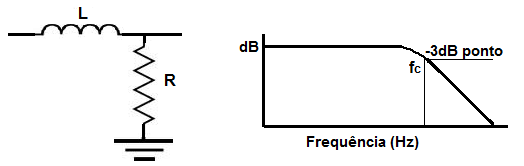
\includegraphics[width=0.9\textwidth]{Imagens/FiltroPassaBaixa.png}
		\legend{Fonte: Produzido pelos autores}
		\label{FiltroPassaBaixa}
\end{minipage}}

\subsection{Filtro Passa Alta}

O filtro passa alta é um filtro que permite a passagem das frequências altas, e atenua (ou reduz) a amplitude das frequências abaixo de frequência de corte ($ f_c $). O filtro passa alta possui um princípio de funcionamento oposto ao do filtro passa baixa. 

Esse filtro é muito utilizado para bloquear as frequências baixas não desejadas em um sinal complexo enquanto permite a passagem das frequências mais altas.


\centerline{\begin{minipage}[c]{\textwidth}
		\centering
		\noindent
		\captionof{figure}{Diagrama Filtro Passa Alta}
		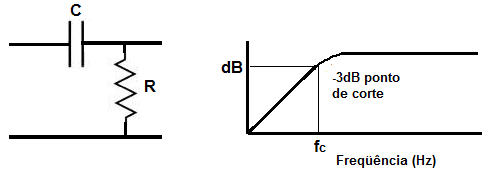
\includegraphics[width=0.9\textwidth]{Imagens/FiltroPassaAlta.png}
		\legend{Fonte: Produzido pelos autores}
		\label{FiltroPassaAlta}
\end{minipage}}

\subsection{Filtro Passa Faixa}

O filtro passa faixa (ou passa-banda) é um circuito elétrico que permite a passagem das frequências de uma certa faixa e rejeita (atenua) as frequências fora dessa faixa. 

Um filtro passa-faixa analógico é o circuito $ RLC $ (um circuito resistor-indutor-capacitor). Tais filtros também podem ser obtidos através da combinação entre um filtro passa-baixas e um filtro passa-altas.

\centerline{\begin{minipage}[c]{\textwidth}
		\centering
		\noindent
		\captionof{figure}{Circuito Passa Faixa}
		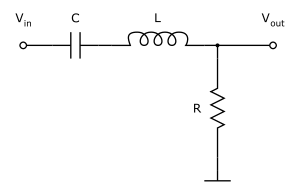
\includegraphics[width=0.5\textwidth]{Imagens/FiltroPassaFaixa1.png}
		\legend{Fonte: Produzido pelos autores}
		\label{FiltroPassaFaixa1}
\end{minipage}}

\centerline{\begin{minipage}[c]{\textwidth}
		\centering
		\noindent
		\captionof{figure}{Diagrama Passa Faixa}
		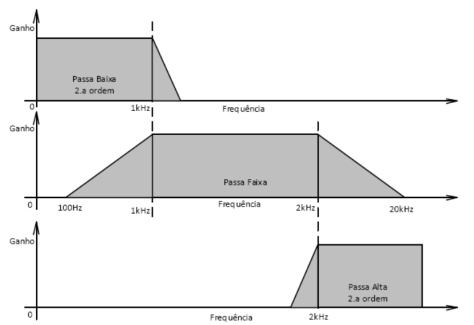
\includegraphics[width=0.9\textwidth]{Imagens/FiltroPassaFaixa2.png}
		\legend{Fonte: Produzido pelos autores}
		\label{FiltroPassaFaixa2}
\end{minipage}}

\subsection{Filtro Rejeita Faixa}
O filtro rejeita faixa ou filtro de rejeição de banda é um filtro que permite a passagem da maioria das frequências inalteradas, porém atenua aquelas que estejam em uma faixa determinada pelo filtro. O princípio de funcionamento é o oposto do filtro passa-faixa.

\centerline{\begin{minipage}[c]{\textwidth}
		\centering
		\noindent
		\captionof{figure}{Circuito Rejeita Faixa}
		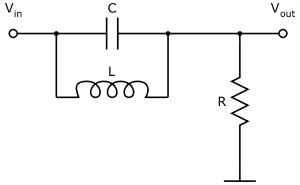
\includegraphics[width=0.5\textwidth]{Imagens/FiltroRejeitaFaixa1.png}
		\legend{Fonte: Produzido pelos autores}
		\label{FiltroRejeitaFaixa1}
\end{minipage}}

\centerline{\begin{minipage}[c]{\textwidth}
		\centering
		\noindent
		\captionof{figure}{Diagrama Rejeita Faixa}
		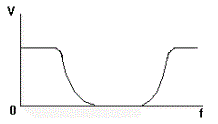
\includegraphics[width=0.4\textwidth]{Imagens/FiltroRejeitaFaixa2.png}
		\legend{Fonte: Produzido pelos autores}
		\label{FiltroRejeitaFaixa2}
\end{minipage}}



\newpage
\section{Procedimentos}


\subsection{Amplificador $ 1^\circ $ estágio}

\centerline{\begin{minipage}[c]{\textwidth}
		\centering
		\noindent
		\captionof{figure}{Circuito elétrico do $ 1^\circ $ estágio do amplificador}
		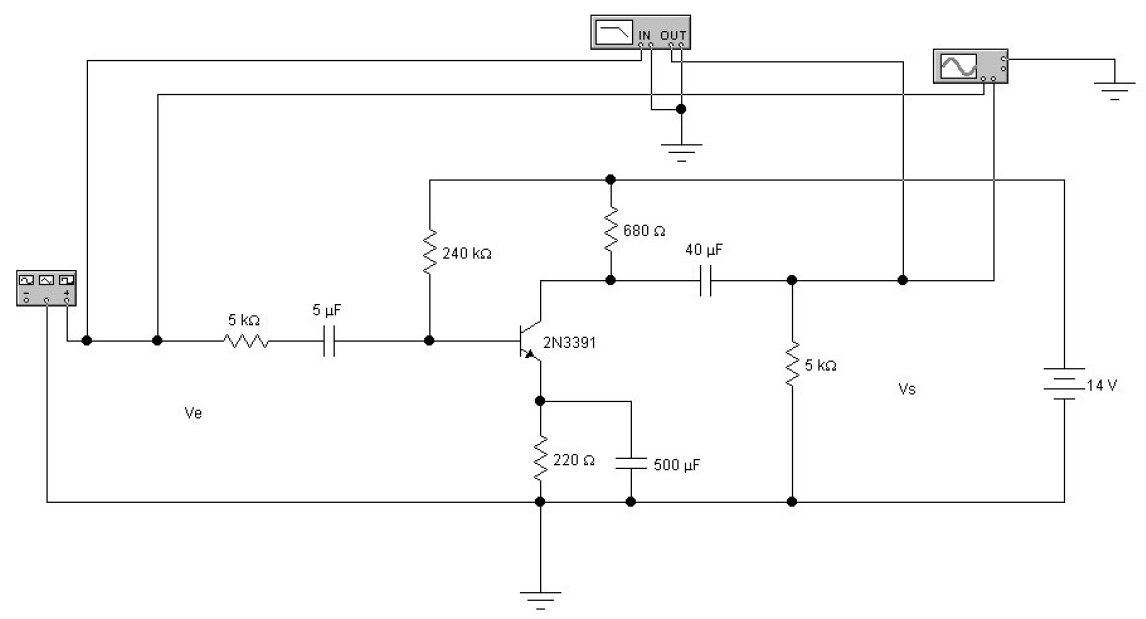
\includegraphics[width=0.9\textwidth]{Imagens/Figura1.jpg}
		\legend{Fonte: Produzido pelos autores}
		\label{Figura1}
\end{minipage}}
	
\begin{enumerate}
	\item Dado o circuito da figura \ref{Figura1}, aplicar o gerador de funções com uma tensão $ 1,0mV $ e frequência de $ 1kHz $;
	\item Medir o ganho com o osciloscópio. Para tanto medir a tensão de saída $ V_s $ e de entrada $ V_e $.
	\item Usar o Bode Plotter (amplitude) e medir as frequências de corte e o ganho da banda passante em $ dB $ $ A $ $ db = 20 \log (V_s/V_e) $;
	\item Usar o Bode Plotter (fase) e medir os ângulos nas frequências importantes; Anotar todos os dados obtidos na tabela \ref{Tabela1}.
\end{enumerate}


\subsection{Amplificador $ 2^\circ $ estágio}

\centerline{\begin{minipage}[c]{\textwidth}
		\centering
		\noindent
		\captionof{figure}{Circuito elétrico do $ 2^\circ $ estágio do amplificador}
		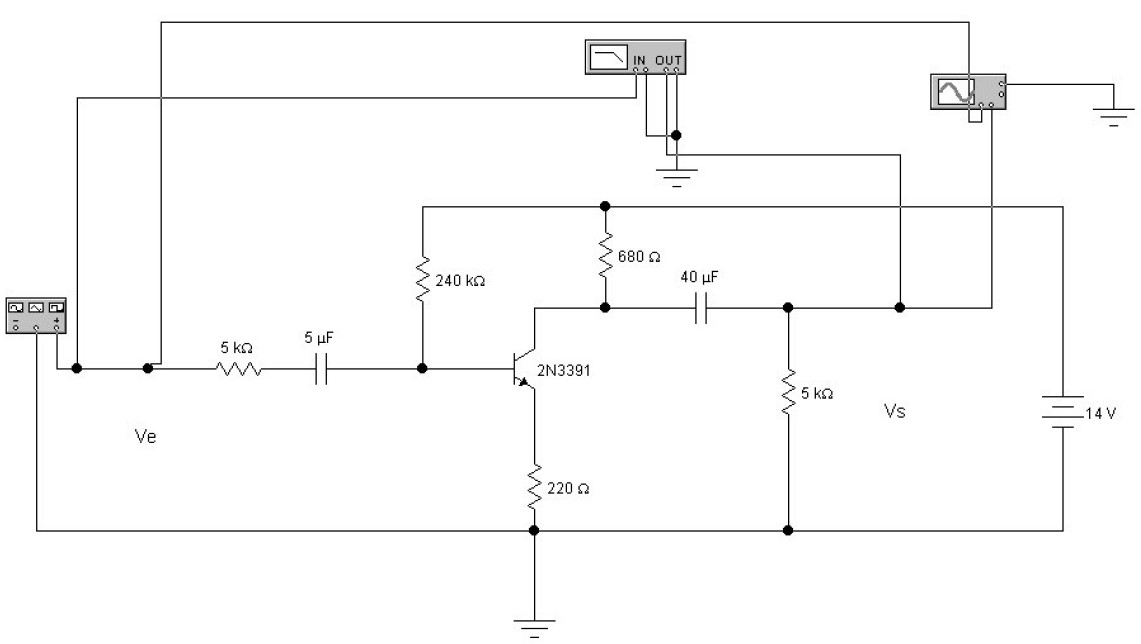
\includegraphics[width=0.9\textwidth]{Imagens/Figura2.jpg}
		\legend{Fonte: Produzido pelos autores}
		\label{Figura2}
\end{minipage}}

\begin{enumerate}
	\item Dado o circuito figura \ref{Figura2}, aplicar o gerador de funções com uma tensão $ 1,0mV $ e frequência de $ 1kHz $;
	\item Medir o ganho com o osciloscópio. Para tanto medir a tensão de saída $ V_s $ e de entrada $ V_e $.
	\item Usar o Bode Plotter (amplitude) e medir as frequências de corte e o ganho da banda passante em $ dB $;
	\item Usar o Bode Plotter (fase) e medir os ângulos nas frequências importantes; Anotar todos os dados obtidos na tabela \ref{Tabela1}.
\end{enumerate}

\subsection{Amplificador com dois estágios}

\centerline{\begin{minipage}[c]{\textwidth}
		\centering
		\noindent
		\captionof{figure}{Circuito elétrico do amplificador com dois estágios}
		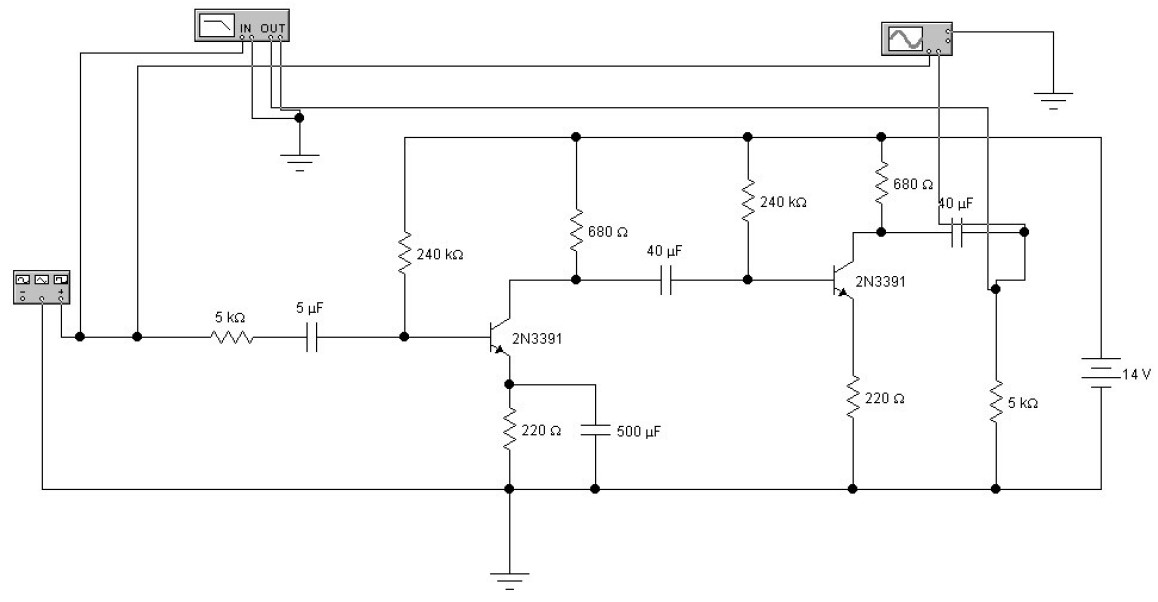
\includegraphics[width=0.9\textwidth]{Imagens/Figura3.jpg}
		\legend{Fonte: Produzido pelos autores}
		\label{Figura3}
\end{minipage}}

\begin{enumerate}
	\item Dado o circuito figura \ref{Figura3}, aplicar o gerador de funções com uma tensão $ 1,0mV $ e frequência de $ 1kHz $;
	\item Medir o ganho com o osciloscópio. Para tanto medir a tensão de saída $ V_s $ e de entrada $ V_e $.
	\item Usar o Bode Plotter (amplitude) e medir as frequências de corte e o ganho da banda passante em $ dB $;
\end{enumerate}

\subsection{Analise}
\begin{enumerate}
	\item Analise os resultados apontados na Tabela \ref{Tabela2} e explique:
	\begin{enumerate}
		\item Por que a frequência de corte inferior $ (fr_1) $ para o circuito da figura \ref{Figura1} é maior que para o circuito da figura \ref{Figura2}?
		\item Por que o ganho, para a faixa de frequência médias, do circuito da figura \ref{Figura1} é bem maior do que o circuito da figura \ref{Figura2}?
	\end{enumerate}
\end{enumerate}

\centerline{\begin{minipage}[c]{\textwidth}
		\centering
		\noindent
		\captionof{table}{Valores obtidos dos circuitos}
		\begin{tabular}{ll|c|c|l|}
			\cline{3-5}
			&     & Circuito $ 1 $ & Circuito $ 2 $ & Circuito $ 3 $ \\ \hline
			\multicolumn{1}{|c|}{\multirow{3}{*}{Osciloscópio}} & $V_e$ $ (V_{pp}) $   &            &            &            \\ \cline{2-5} 
			\multicolumn{1}{|c|}{}                              & $V_s$ $ (V_{pp}) $   &            &            &            \\ \cline{2-5} 
			\multicolumn{1}{|c|}{}                              & $A_V$ $ (V_s/V_e) $   &            &            &            \\ \hline
			\multicolumn{1}{|l|}{\multirow{3}{*}{Bode Plotter}} & $A_V$ em frequências médias $ (dB) $   &            &            &            \\ \cline{2-5} 
			\multicolumn{1}{|l|}{}                              & frequência $ 1 $ a $ (-3dB) $ &            &            &            \\ \cline{2-5} 
			\multicolumn{1}{|l|}{}                              & frequência $ 2 $ a $ (-3dB) $ &            &            &            \\ \hline
		\end{tabular}
		\legend{Fonte: Produzido pelos autores}
		\label{Tabela1}
\end{minipage}}

\newpage
\section{Resultados}

\subsection{Amplificador $ 1^\circ $ estágio}
Temos a seguinte montagem do circuito da figura \ref{Figura1} com a utilização do MULTISIM:


\begin{center}
	\textbf{--- ADD a imagem - Simulação\_Circuito1.png ---}
\end{center}

Com a utilização do Osciloscópio do simulador, conseguimos obter a forma de onda da entrada e da saída, que para uma melhor visualização deixando as duas formas de onda com escalas diferentes.

\centerline{\begin{minipage}[c]{\textwidth}
		\centering
		\noindent
		\captionof{figure}{Imagem do osciloscópio do Circuito \ref{Figura1}}
		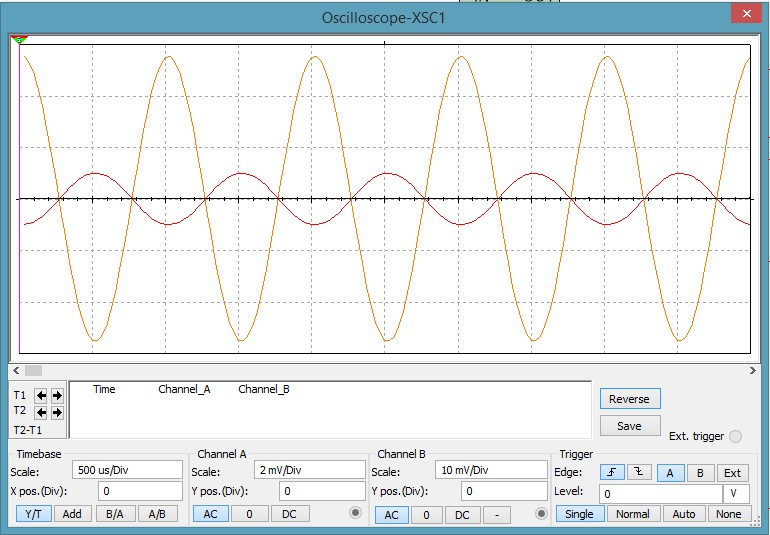
\includegraphics[width=0.9\textwidth]{Imagens/Oscilloscope_Circuito1.jpg}
		\legend{Fonte: Produzido pelos autores}
		\label{Oscilloscope_Circuito1}
\end{minipage}}

Usando o Bode Plotter, conseguimos analisar o gráfico do ganho em relação a frequência do circuito.

\centerline{\begin{minipage}[c]{\textwidth}
		\centering
		\noindent
		\captionof{figure}{Bode Plotter do Circuito \ref{Figura1}}
		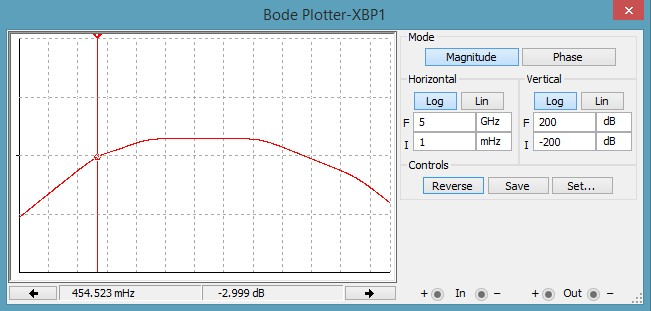
\includegraphics[width=0.9\textwidth]{Imagens/BodePlotter_Circuito1_Parte1.jpg}
		\legend{Fonte: Produzido pelos autores}
		\label{BodePlotter_Circuito1_Parte1}
\end{minipage}}

\centerline{\begin{minipage}[c]{\textwidth}
		\centering
		\noindent
		\captionof{figure}{Bode Plotter do Circuito \ref{Figura1}}
		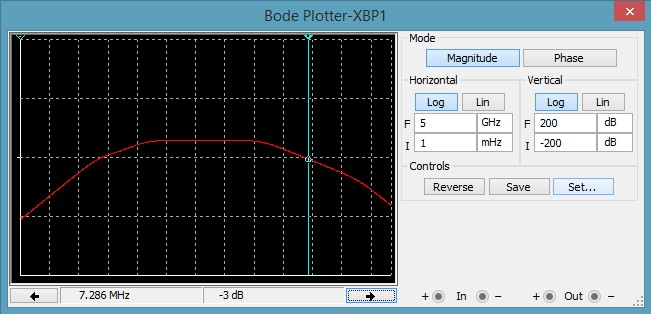
\includegraphics[width=0.9\textwidth]{Imagens/BodePlotter_Circuito1_Parte2.jpg}
		\legend{Fonte: Produzido pelos autores}
		\label{BodePlotter_Circuito1_Parte2}
\end{minipage}}

Com as informações encontradas, obtemos a seguintes informações:

\centerline{\begin{minipage}[c]{\textwidth}
		\centering
		\noindent
		\captionof{table}{Valores obtidos do circuito \ref{Figura1}}
	\begin{tabular}{ll|c|}
		\cline{3-3}
		&     & Circuito 1 \\ \hline
		\multicolumn{1}{|c|}{\multirow{3}{*}{Osciloscópio}} &  $V_e$ $ (V_{pp}) $    &   $ 2mV $         \\ \cline{2-3} 
		\multicolumn{1}{|c|}{}                              & $V_s$ $ (V_{pp}) $   &       $ 55,1mV $     \\ \cline{2-3} 
		\multicolumn{1}{|c|}{}                              &  $A_V$ $ (V_s/V_e) $   &      $ 27,55 $      \\ \hline
		\multicolumn{1}{|l|}{\multirow{3}{*}{Bode Plotter}} & $A_V$ em frequências médias $ (dB) $   &       $ 28,8 dB $     \\ \cline{2-3} 
		\multicolumn{1}{|l|}{}                              & frequência $ 1 $ a $ (-3dB) $ &      $ 454,523mHz  $  \\ \cline{2-3} 
		\multicolumn{1}{|l|}{}                              & frequência $ 2 $ a $ (-3dB) $ &        $ 7,286MHz $    \\ \hline
	\end{tabular}
		\legend{Fonte: Produzido pelos autores}
		\label{Tab_Circuito1}
\end{minipage}}

\subsection{Amplificador $ 2^\circ $ estágio}
Temos a seguinte montagem do circuito da figura \ref{Figura2} com a utilização do MULTISIM:


\begin{center}
	\textbf{--- ADD a imagem - Simulação\_Circuito2.png ---}
\end{center}

Com a utilização do Osciloscópio do simulador, conseguimos obter a forma de onda da entrada e da saída, que para uma melhor visualização deixando as duas formas de onda com escalas diferentes.


\centerline{\begin{minipage}[c]{\textwidth}
		\centering
		\noindent
		\captionof{figure}{Imagem do osciloscópio do Circuito \ref{Figura2}}
		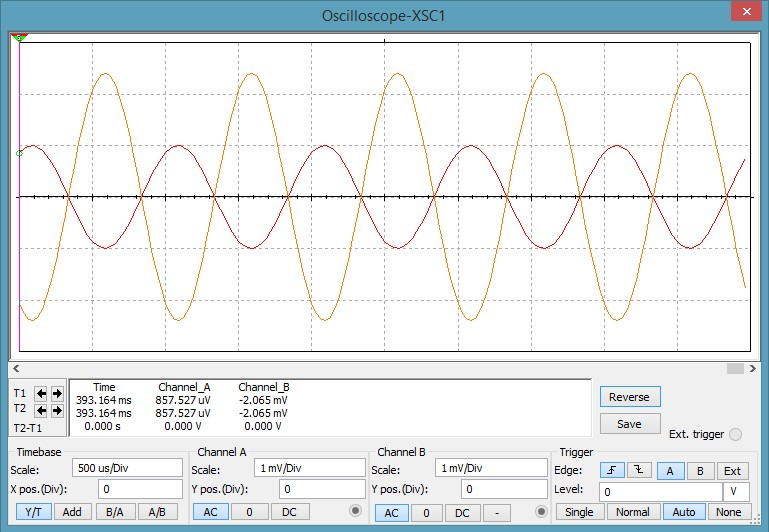
\includegraphics[width=0.9\textwidth]{Imagens/Oscilloscope_Circuito2.jpg}
		\legend{Fonte: Produzido pelos autores}
		\label{Oscilloscope_Circuito2}
\end{minipage}}

Usando o Bode Plotter, conseguimos analisar o gráfico do ganho em relação a frequência do circuito.

\centerline{\begin{minipage}[c]{\textwidth}
		\centering
		\noindent
		\captionof{figure}{Bode Plotter do Circuito \ref{Figura2}}
		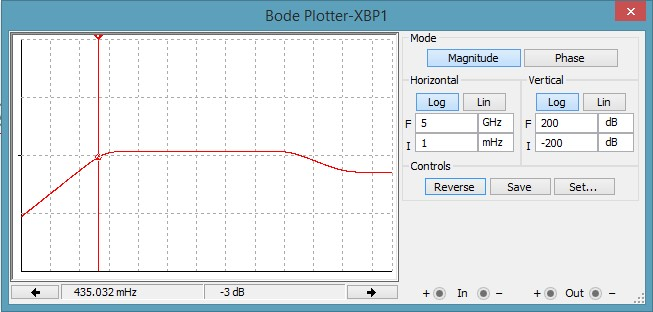
\includegraphics[width=0.9\textwidth]{Imagens/BodePlotter_Circuito2_Parte1.jpg}
		\legend{Fonte: Produzido pelos autores}
		\label{BodePlotter_Circuito2_Parte1}
\end{minipage}}

\centerline{\begin{minipage}[c]{\textwidth}
		\centering
		\noindent
		\captionof{figure}{Bode Plotter do Circuito \ref{Figura2}}
		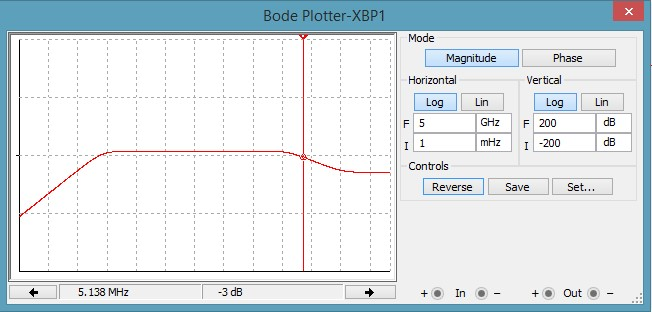
\includegraphics[width=0.9\textwidth]{Imagens/BodePlotter_Circuito2_Parte2.jpg}
		\legend{Fonte: Produzido pelos autores}
		\label{BodePlotter_Circuito2_Parte2}
\end{minipage}}

Com as informações encontradas, obtemos a seguintes informações:

\centerline{\begin{minipage}[c]{\textwidth}
		\centering
		\noindent
		\captionof{table}{Valores obtidos do circuito \ref{Figura2}}
		\begin{tabular}{ll|c|}
			\cline{3-3}
			&     & Circuito 2 \\ \hline
			\multicolumn{1}{|c|}{\multirow{3}{*}{Osciloscópio}} &  $V_e$ $ (V_{pp}) $    &   $ 2mV $         \\ \cline{2-3} 
			\multicolumn{1}{|c|}{}                              & $V_s$ $ (V_{pp}) $   &       $ 4,81mV $     \\ \cline{2-3} 
			\multicolumn{1}{|c|}{}                              &  $A_V$ $ (V_s/V_e) $   &      $ 2,405 $      \\ \hline
			\multicolumn{1}{|l|}{\multirow{3}{*}{Bode Plotter}} & $A_V$ em frequências médias $ (dB) $   &       $ 7,62 dB $     \\ \cline{2-3} 
			\multicolumn{1}{|l|}{}                              & frequência $ 1 $ a $ (-3dB) $ &      $ 435,032mHz  $  \\ \cline{2-3} 
			\multicolumn{1}{|l|}{}                              & frequência $ 2 $ a $ (-3dB) $ &        $ 5,138MHz $    \\ \hline
		\end{tabular}
		\legend{Fonte: Produzido pelos autores}
		\label{Tab_Circuito2}
\end{minipage}}

\subsection{Amplificador com dois estágios}

Temos a seguinte montagem do circuito da figura \ref{Figura3} com a utilização do MULTISIM:


\begin{center}
	\textbf{--- ADD a imagem - Simulação\_Circuito3.png ---}
\end{center}

Com a utilização do Osciloscópio do simulador, conseguimos obter a forma de onda da entrada e da saída, que para uma melhor visualização deixando as duas formas de onda com escalas diferentes.

\centerline{\begin{minipage}[c]{\textwidth}
		\centering
		\noindent
		\captionof{figure}{Imagem do osciloscópio do Circuito \ref{Figura3}}
		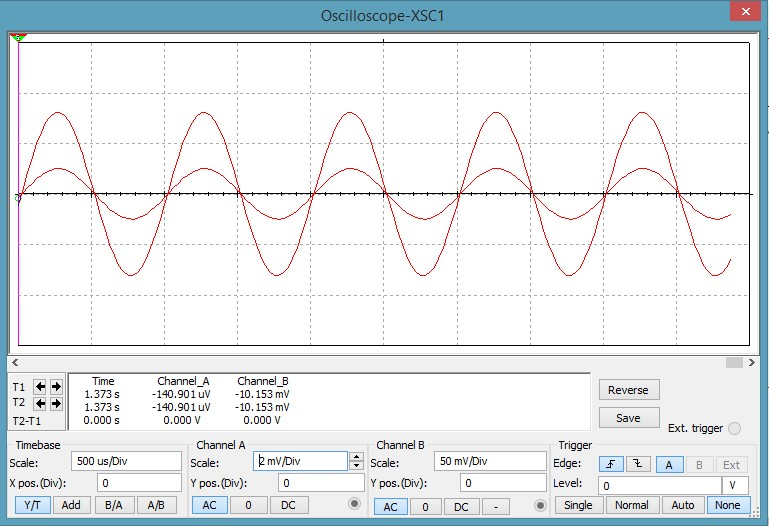
\includegraphics[width=0.9\textwidth]{Imagens/Oscilloscope_Circuito3.jpg}
		\legend{Fonte: Produzido pelos autores}
		\label{Oscilloscope_Circuito3}
\end{minipage}}

Usando o Bode Plotter, conseguimos analisar o gráfico do ganho em relação a frequência do circuito.

\centerline{\begin{minipage}[c]{\textwidth}
		\centering
		\noindent
		\captionof{figure}{Bode Plotter do Circuito \ref{Figura3}}
		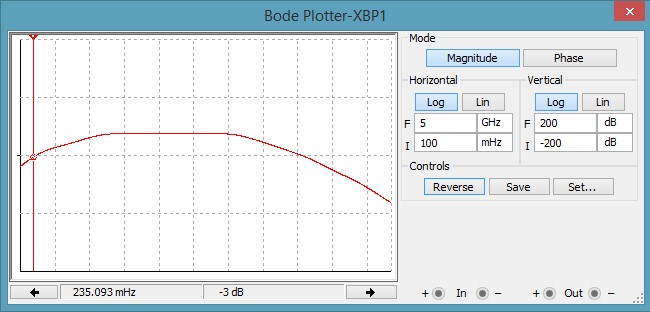
\includegraphics[width=0.9\textwidth]{Imagens/BodePlotter_Circuito3_Parte1.jpg}
		\legend{Fonte: Produzido pelos autores}
		\label{BodePlotter_Circuito3_Parte1}
\end{minipage}}

\centerline{\begin{minipage}[c]{\textwidth}
		\centering
		\noindent
		\captionof{figure}{Bode Plotter do Circuito \ref{Figura3}}
		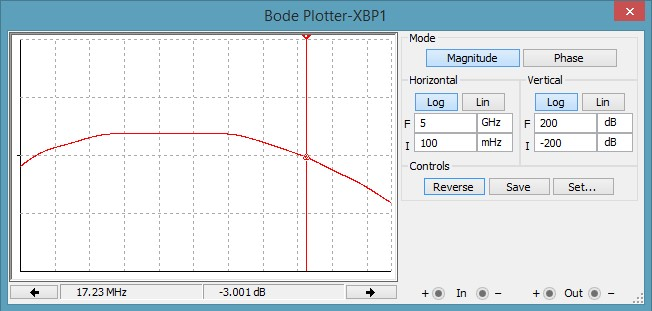
\includegraphics[width=0.9\textwidth]{Imagens/BodePlotter_Circuito3_Parte2.jpg}
		\legend{Fonte: Produzido pelos autores}
		\label{BodePlotter_Circuito3_Parte2}
\end{minipage}}

Com as informações encontradas, obtemos a seguintes informações:

\centerline{\begin{minipage}[c]{\textwidth}
		\centering
		\noindent
		\captionof{table}{Valores obtidos do circuito \ref{Figura3}}
		\begin{tabular}{ll|c|}
			\cline{3-3}
			&     & Circuito 3 \\ \hline
			\multicolumn{1}{|c|}{\multirow{3}{*}{Osciloscópio}} &  $V_e$ $ (V_{pp}) $    &   $ 2mV $         \\ \cline{2-3} 
			\multicolumn{1}{|c|}{}                              & $V_s$ $ (V_{pp}) $   &       $ 162mV $     \\ \cline{2-3} 
			\multicolumn{1}{|c|}{}                              &  $A_V$ $ (V_s/V_e) $   &      $ 81 $      \\ \hline
			\multicolumn{1}{|l|}{\multirow{3}{*}{Bode Plotter}} & $A_V$ em frequências médias $ (dB) $   &       $ 38,17 dB $     \\ \cline{2-3} 
			\multicolumn{1}{|l|}{}                              & frequência $ 1 $ a $ (-3dB) $ &      $ 235,093mHz  $  \\ \cline{2-3} 
			\multicolumn{1}{|l|}{}                              & frequência $ 2 $ a $ (-3dB) $ &        $ 17,23MHz $    \\ \hline
		\end{tabular}
		\legend{Fonte: Produzido pelos autores}
		\label{Tab_Circuito3}
\end{minipage}}

\subsection{Análise}
Para facilitar a análise, juntamos as informações obtidas de cada circuito numa tabela só.

\centerline{\begin{minipage}[c]{\textwidth}
		\centering
		\noindent
		\captionof{table}{Valores obtidos dos circuitos}
		\begin{tabular}{ll|c|c|c|}
			\cline{3-5}
			&     & Circuito $ 1 $ & Circuito $ 2 $ & Circuito $ 3 $ \\ \hline
			\multicolumn{1}{|c|}{\multirow{3}{*}{Osciloscópio}} & $V_e$ $ (V_{pp}) $   &$ 2mV $&$ 2mV $&$ 2mV $\\ \cline{2-5} 
			\multicolumn{1}{|c|}{}                              & $V_s$ $ (V_{pp}) $   &$ 55,1mV $&$ 4,81mV $&$ 162mV $            \\ \cline{2-5} 
			\multicolumn{1}{|c|}{}                              & $A_V$ $ (V_s/V_e) $   &$ 27,55 $&$ 2,405 $&   $ 81 $         \\ \hline
			\multicolumn{1}{|l|}{\multirow{3}{*}{Bode Plotter}} & $A_V$ em frequências médias &$ 28,8dB $&$ 7,62dB $ &$ 38,17 dB $ \\ \cline{2-5} 
			\multicolumn{1}{|l|}{}                              & frequência $ 1 $ a $ (-3dB) $ &$ 454,523mHz $&$ 435,032mHz $& $ 235,093mHz  $  \\ \cline{2-5} 
			\multicolumn{1}{|l|}{}                              & frequência $ 2 $ a $ (-3dB) $ &$ 7,286MHz $&$ 5,138MHz $& $ 17,23MHz $ \\ \hline
		\end{tabular}
		\legend{Fonte: Produzido pelos autores}
		\label{Tabela2}
\end{minipage}}

\begin{enumerate}
	\item Analise os resultados apontados na Tabela \ref{Tabela2} e explique:
	\begin{enumerate}
		\item Por que a frequência de corte inferior $ (fr_1) $ para o circuito da figura \ref{Figura1} é maior que para o circuito da figura \ref{Figura2}?
		
		\textit{A diferença do circuito da figura \ref{Figura1} para a figura \ref{Figura2} é que possui um capacitor de $ 500 \mu F $ na saída do emissor, fazendo assim um filtro de passa baixa, aumentando a frequência de corte do circuito da figura \ref{Figura1}.}
		
		\item Por que o ganho, para a faixa de frequência médias, do circuito da figura \ref{Figura1} é bem maior do que o circuito da figura \ref{Figura2}?
		
		\textit{Com capacitor adicionado da figura \ref{Figura1} na saída do emissor, temos que quando o transistor está trabalhando em corrente alternada, por ser de alta frequência em $ CA $, temos que o capacitor se assemelha a um curto circuito, fazendo com que o $ R_E $ que não interfira no circuito, havendo assim uma impedância de entrada menor, onde a corrente de entrada ($ I_B $) é maior, fazendo com que a impedância de saída seja maior. Já na figura \ref{Figura2} sem o capacitor no emissor, faz com que em $ CA $ o circuito tenha uma impedância de entrada muito maior, por causa do aparecimento do $ R_E $, fazendo com que tenha uma corrente de entrada menor ($ I_B $), onde influencia na impedância de saída, fazendo com que fique menor. Consequentemente o ganho do circuito da figura \ref{Figura1} é bem maior do que o circuito da figura \ref{Figura2}}
		
	\end{enumerate}
\end{enumerate}



